% ==============================================================================
% INTRO SECTION
% Motivation and research question
% ==============================================================================

% ==============================================================================
% SLIDE: MOTIVATION
% ==============================================================================
\begin{frame}
    \frametitle{Motivation}

    \begin{itemize}
        \item Lots of current policy debate about the appropriate level of decentralization in land-use decision-making
        \begin{itemize}
            \item In the US, hyperlocal land-use decisions have become very common but potentially overweight incumbent preferences relative to aggregate welfare
            \citep{fischel_homevoter_2009,ortalo-magne_political_2014,been_urban_2014, khan_decentralized_2021,fang_homeowner_2023,mast_warding_2024}
            \item However, top-down decision-making can also ignore local preferences for density and congestion, and hurt wealth-building through lower housing prices \cite{jacobs_life_1961,gyourko_distaste_2024}
        \end{itemize}
        \item Theoretically ambiguous which level of centralization is ``optimal'' and may depend on how a social planner weights incumbents vs. new residents, and how much local information is relevant for land-use decisions
    \end{itemize}
\end{frame}

% ==============================================================================
% SLIDE: News Examples
% ==============================================================================

\begin{frame}
	\frametitle{Local Control is a Hot Topic Amongst Policymakers and Academics}
    \begin{minipage}{0.5\textwidth}
        \begin{figure}
            \centering
            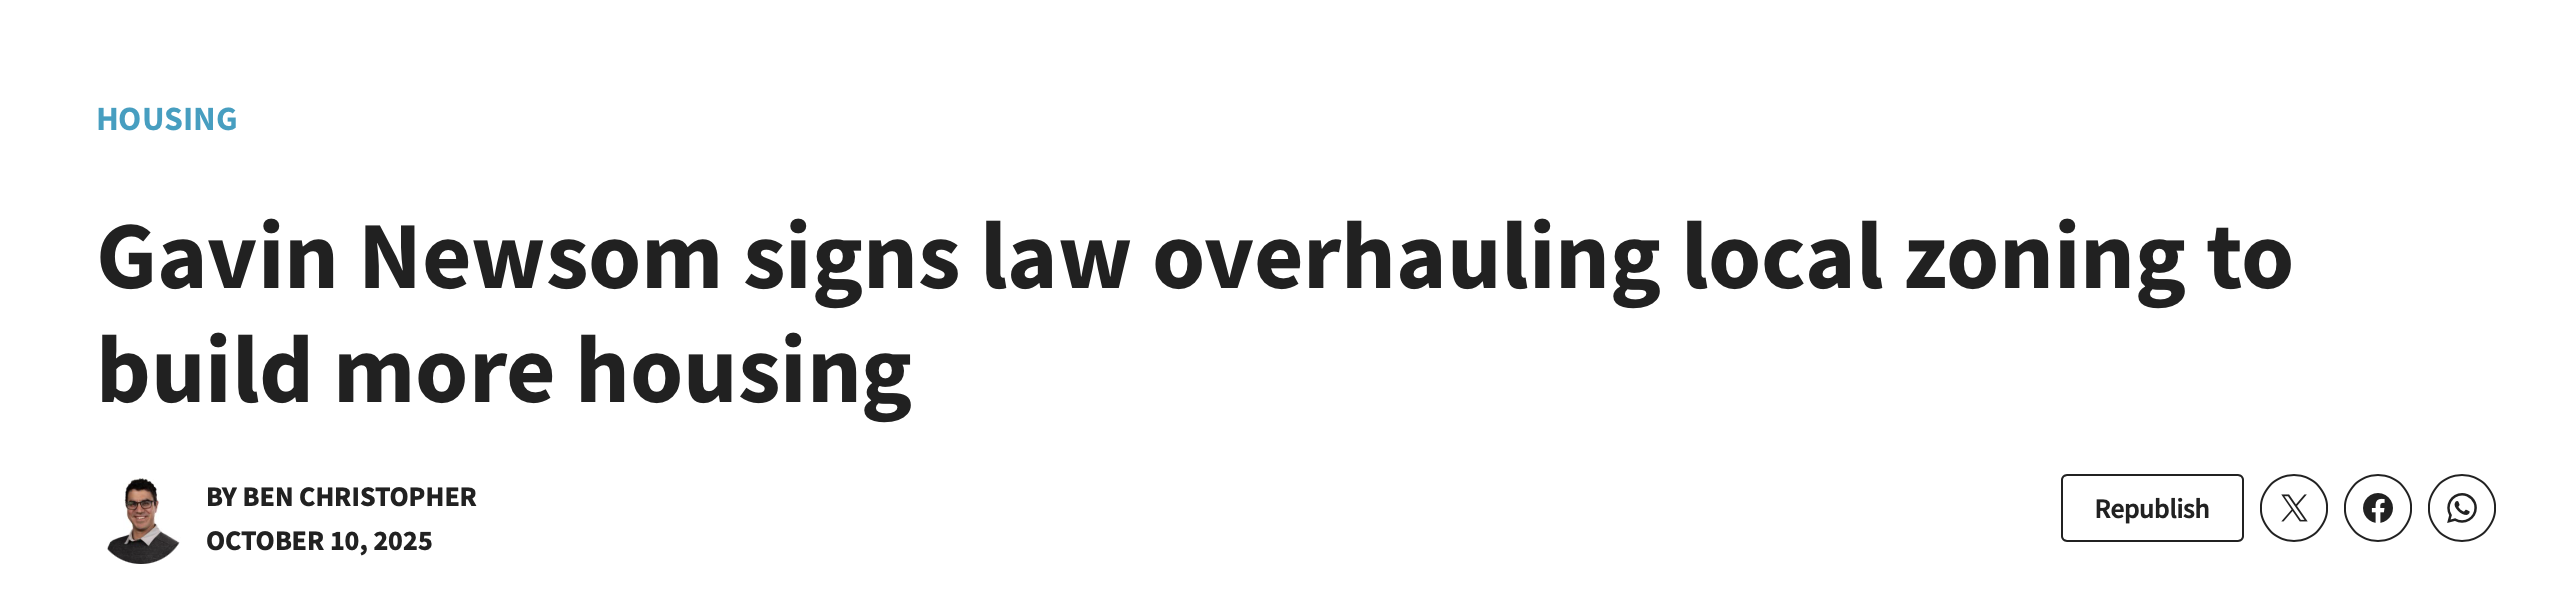
\includegraphics[width=\textwidth]{images/california_local_control.png}
		\end{figure}
		\begin{figure}
			\centering
			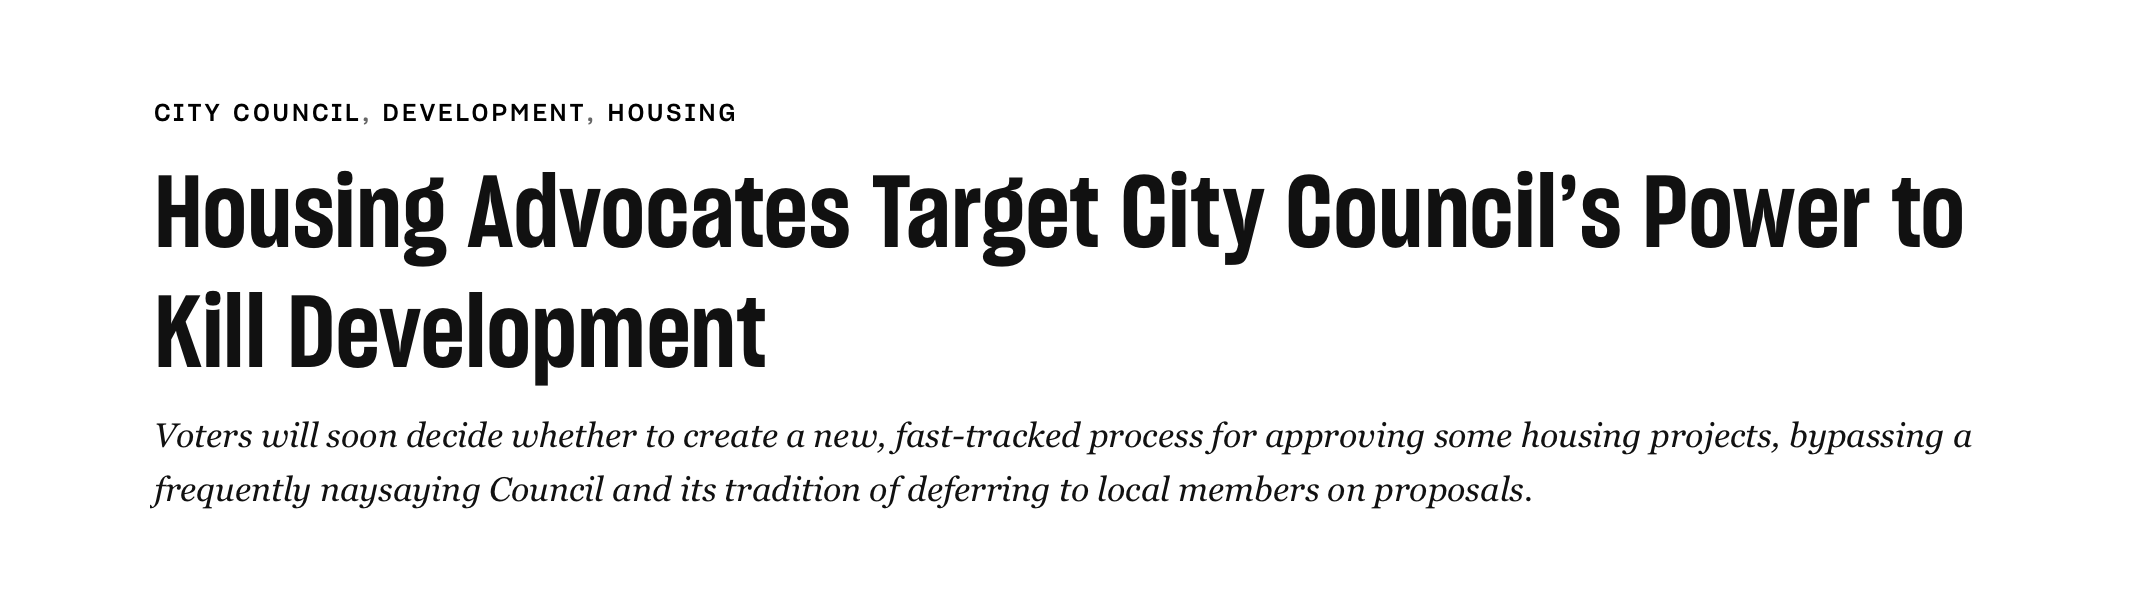
\includegraphics[width=\textwidth]{images/nyc_member_deference.png}
		\end{figure}
		\begin{figure}
			\centering
			
\includegraphics[width=\textwidth]{images/illinois_local_control_pritzker.png}
		\end{figure}
        \end{minipage}
        \hfill
        \begin{minipage}{0.48\textwidth}
        \begin{figure}
            \centering
            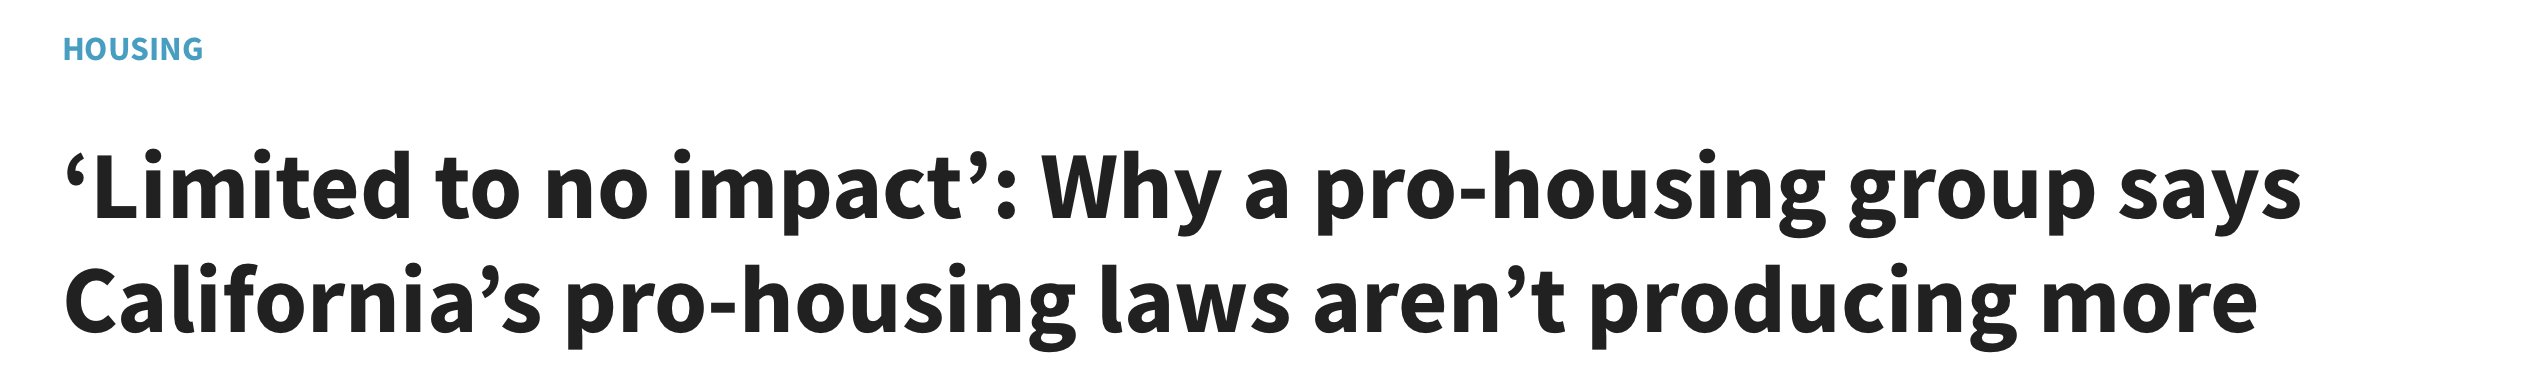
\includegraphics[width=\textwidth]{images/california_ineffective.png}
		\end{figure}
		\begin{figure}
			\centering
			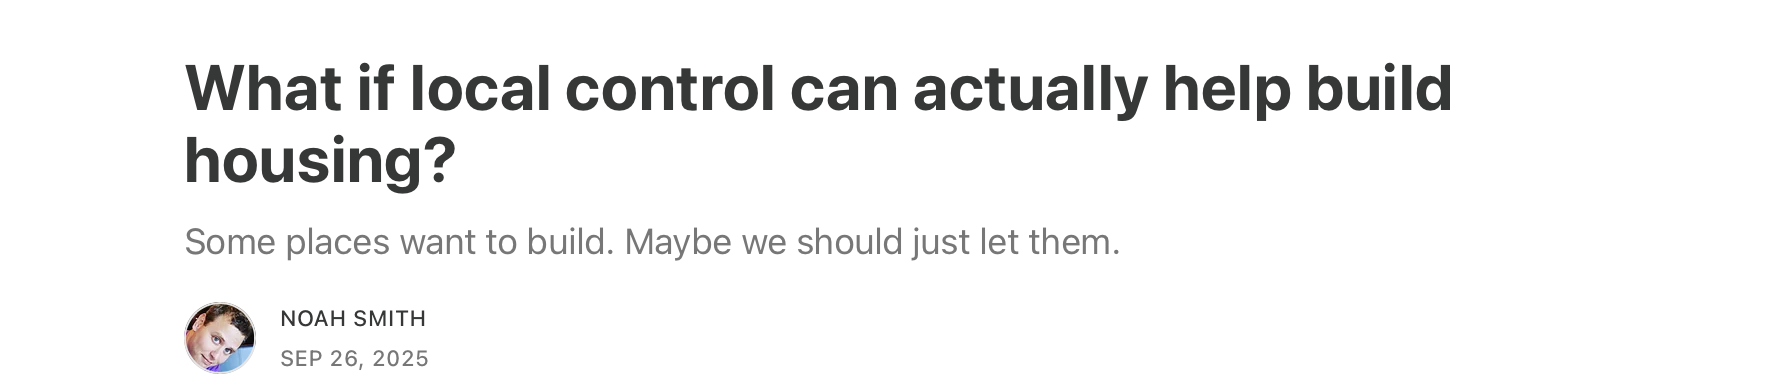
\includegraphics[width=\textwidth]{images/local_control_good_noah_smith.png}
        \end{figure}
        \end{minipage}
\end{frame}
% ==============================================================================
% SLIDE: THIS PAPER
% ==============================================================================
\begin{frame}
    \frametitle{This Paper}
    \textbf{Research question}: What are the welfare effects of centralizing land-use decision-making? Who gains and who loses from local control? \\
    \textbf{This paper:}
    \begin{itemize}
        \item Use a 1989 Supreme Court case in New York City (\textit{Board of Estimate v. Morris}) that shifted land-use decision-making from a citywide board to 51 city council districts
        \item I find that the shift to local control substantially reallocated new housing supply in the city relative to before 1990
        \item Develop a quantitative spatial model of land-use regulation to estimate the welfare effects of local control and the importance of local information in land-use decisions
    \end{itemize}
\end{frame}

\begin{frame}
    \frametitle{Setting: New York City}
    \begin{itemize}
        \item 1989 Supreme Court case \textit{Board of Estimate v. Morris} ruled current land-use regime unconstitutional
        \item Shifted land-use decision-making from a citywide board (the Board of Estimate) to the 51 city council districts
        \item Board of Estimate
    \begin{itemize}
        \item 11 votes: 2 for mayor, 2 for comptroller, 2 for president of the city council, and one for each of the 5 borough presidents
        \item In practice, the mayor made most land-use decisions resulting in a centralized regime
    \end{itemize}
    \end{itemize}
\end{frame}
